\begin{frame}
    \frametitle{Научная новизна}
    \begin{enumerate}
        \item Доказано, что правильные семейства булевых функций находятся во взаимно-однозначном соответствии с одностоковыми ориентациями графов булевых кубов;
        \item Показано, что отображения, задаваемые с помощью правильных семейств булевых функций, всегда имеют четное число неподвижных точек;
        \item Получена нижняя оценка на число правильных семейств булевых функций;
        \item Предложены оценки доли треугольных семейств среди всех правильных семейств булевых функций;
        \item Обнаружен новый класс правильных семейств булевых функций, доказана его правильность;
        \item Предложен новый алгоритм шифрования, основанный на квазигрупповых операциях;
    \end{enumerate}
\end{frame}


\begin{frame}
    \frametitle{Отзыв на НКР-1}
    \centering
    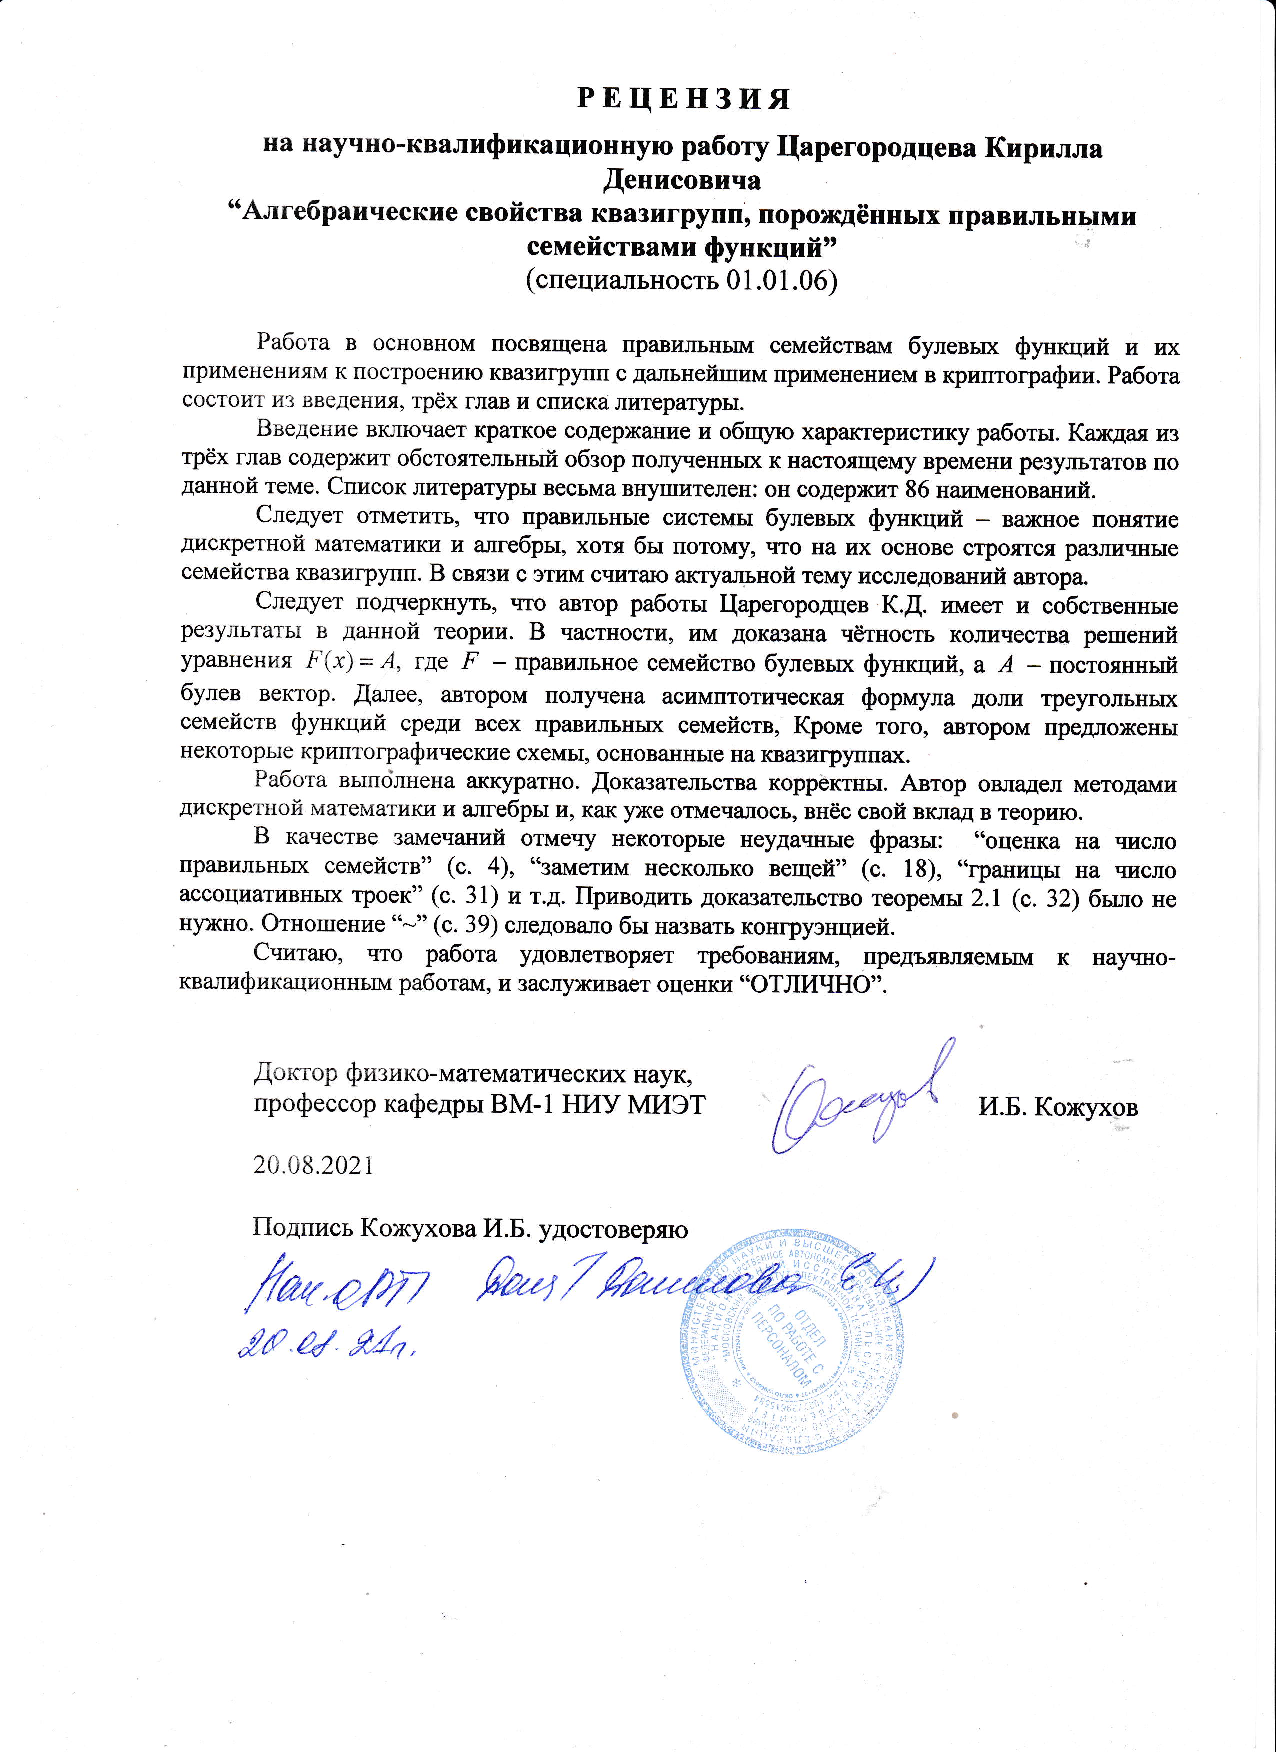
\includegraphics[width=0.7\linewidth]{review_outer}
\end{frame}

\begin{frame}
    \frametitle{Отзыв на НКР-2}
    \centering
    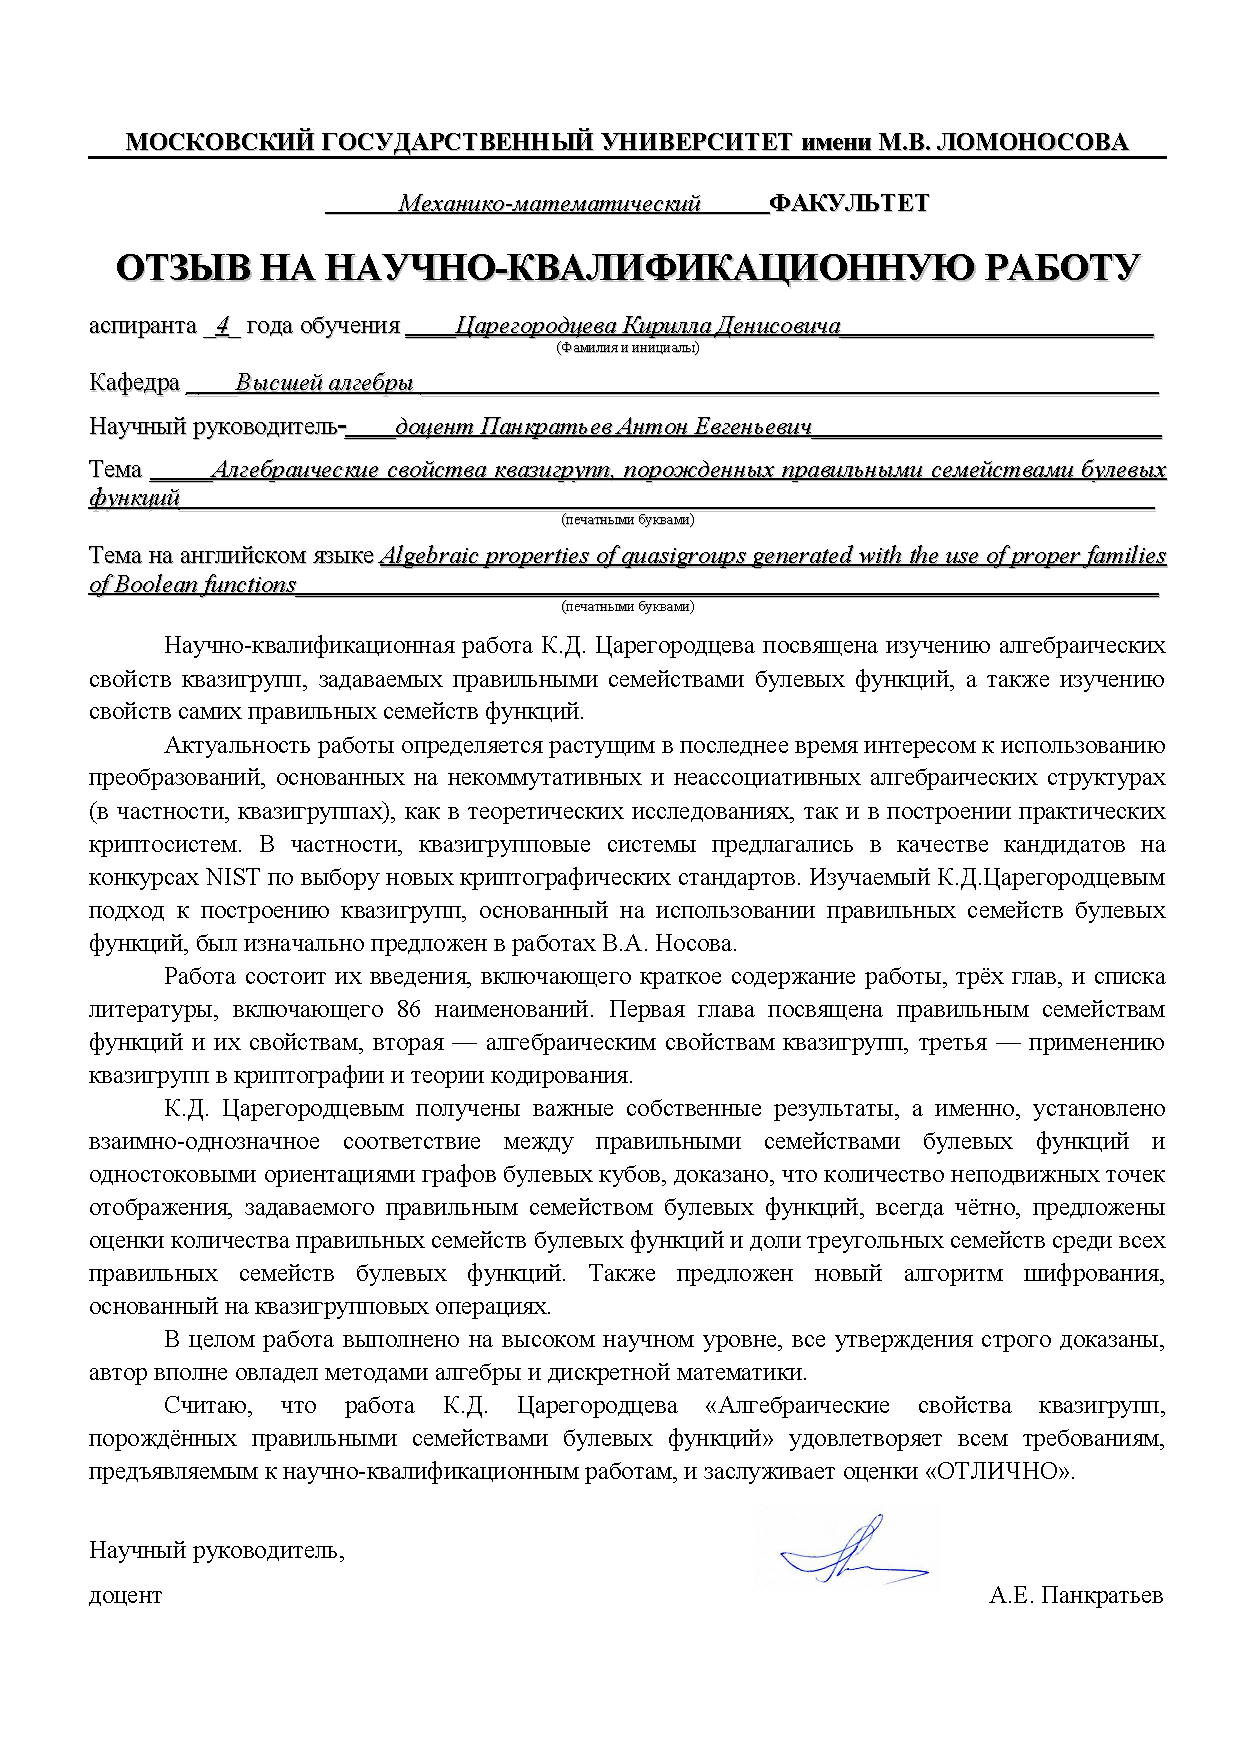
\includegraphics[width=0.6\linewidth]{review_inner}
\end{frame}

\begin{frame}
    \frametitle{Заключение кафедры}
    \centering
    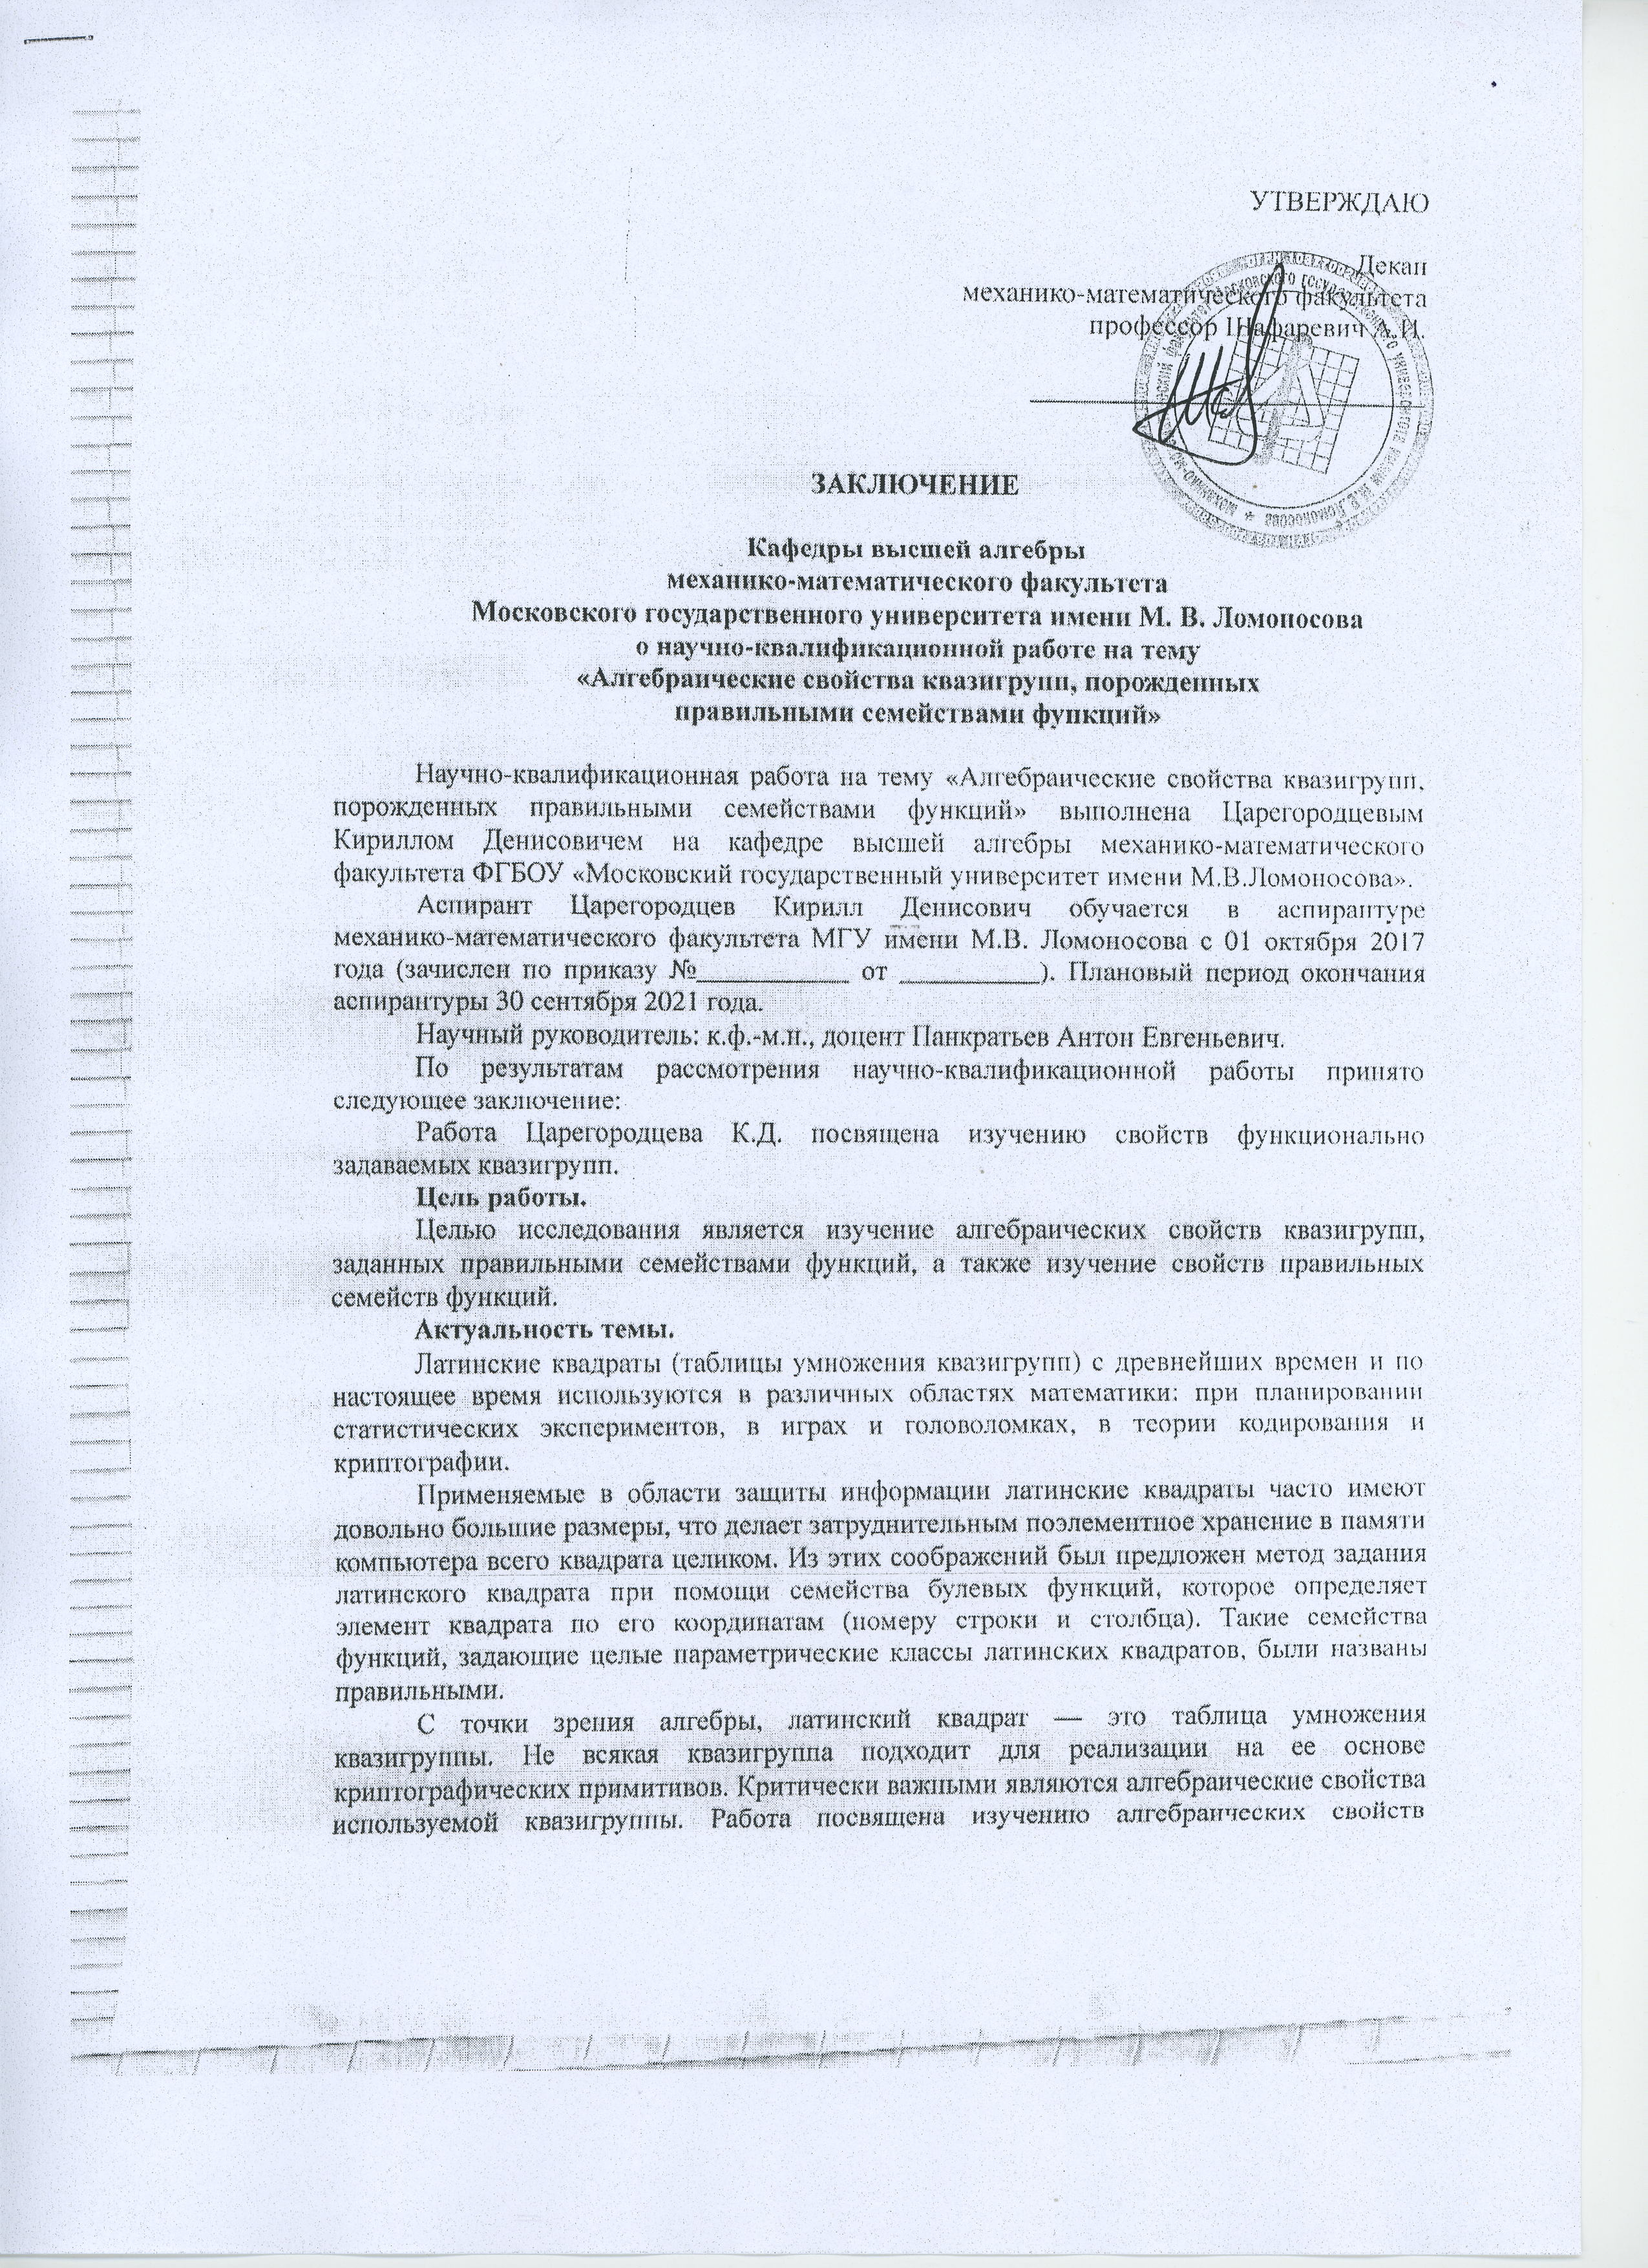
\includegraphics[width=0.65\linewidth]{kaf1}
\end{frame}

\begin{frame}
    \frametitle{Заключение кафедры}
    \centering
    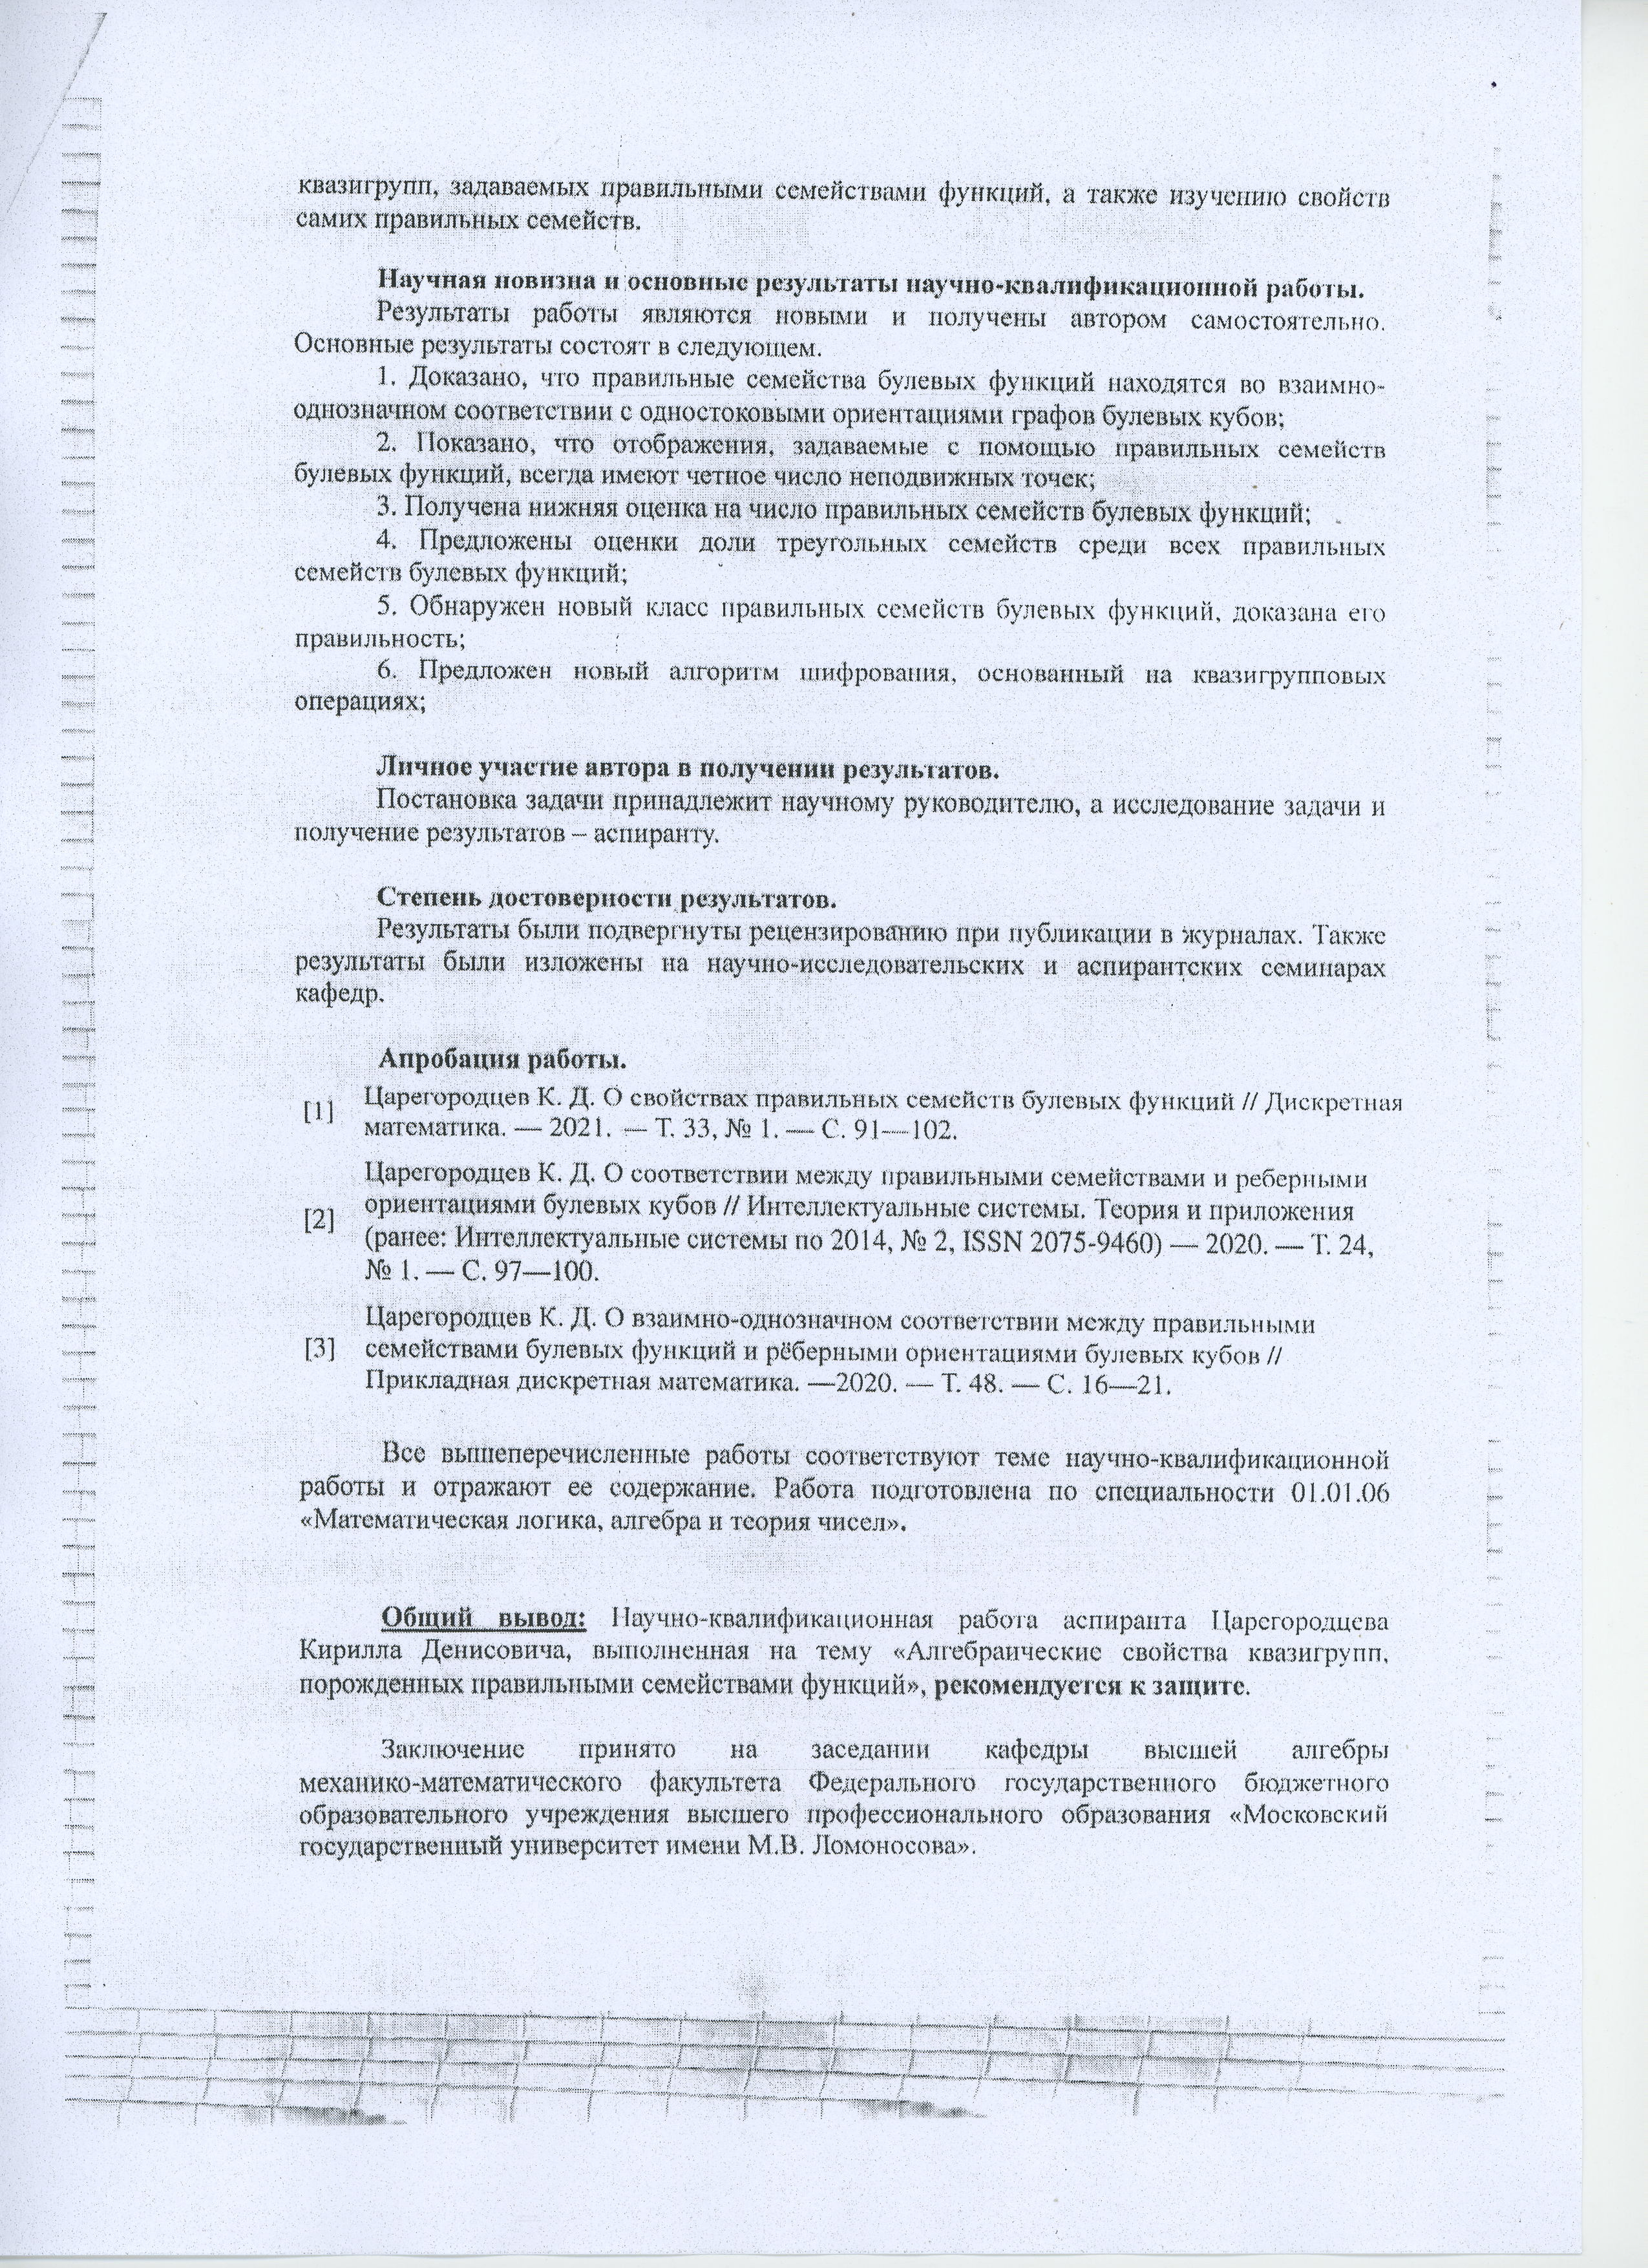
\includegraphics[width=0.65\linewidth]{kaf2}
\end{frame}

\begin{frame}
    \frametitle{Заключение кафедры}
    \centering
    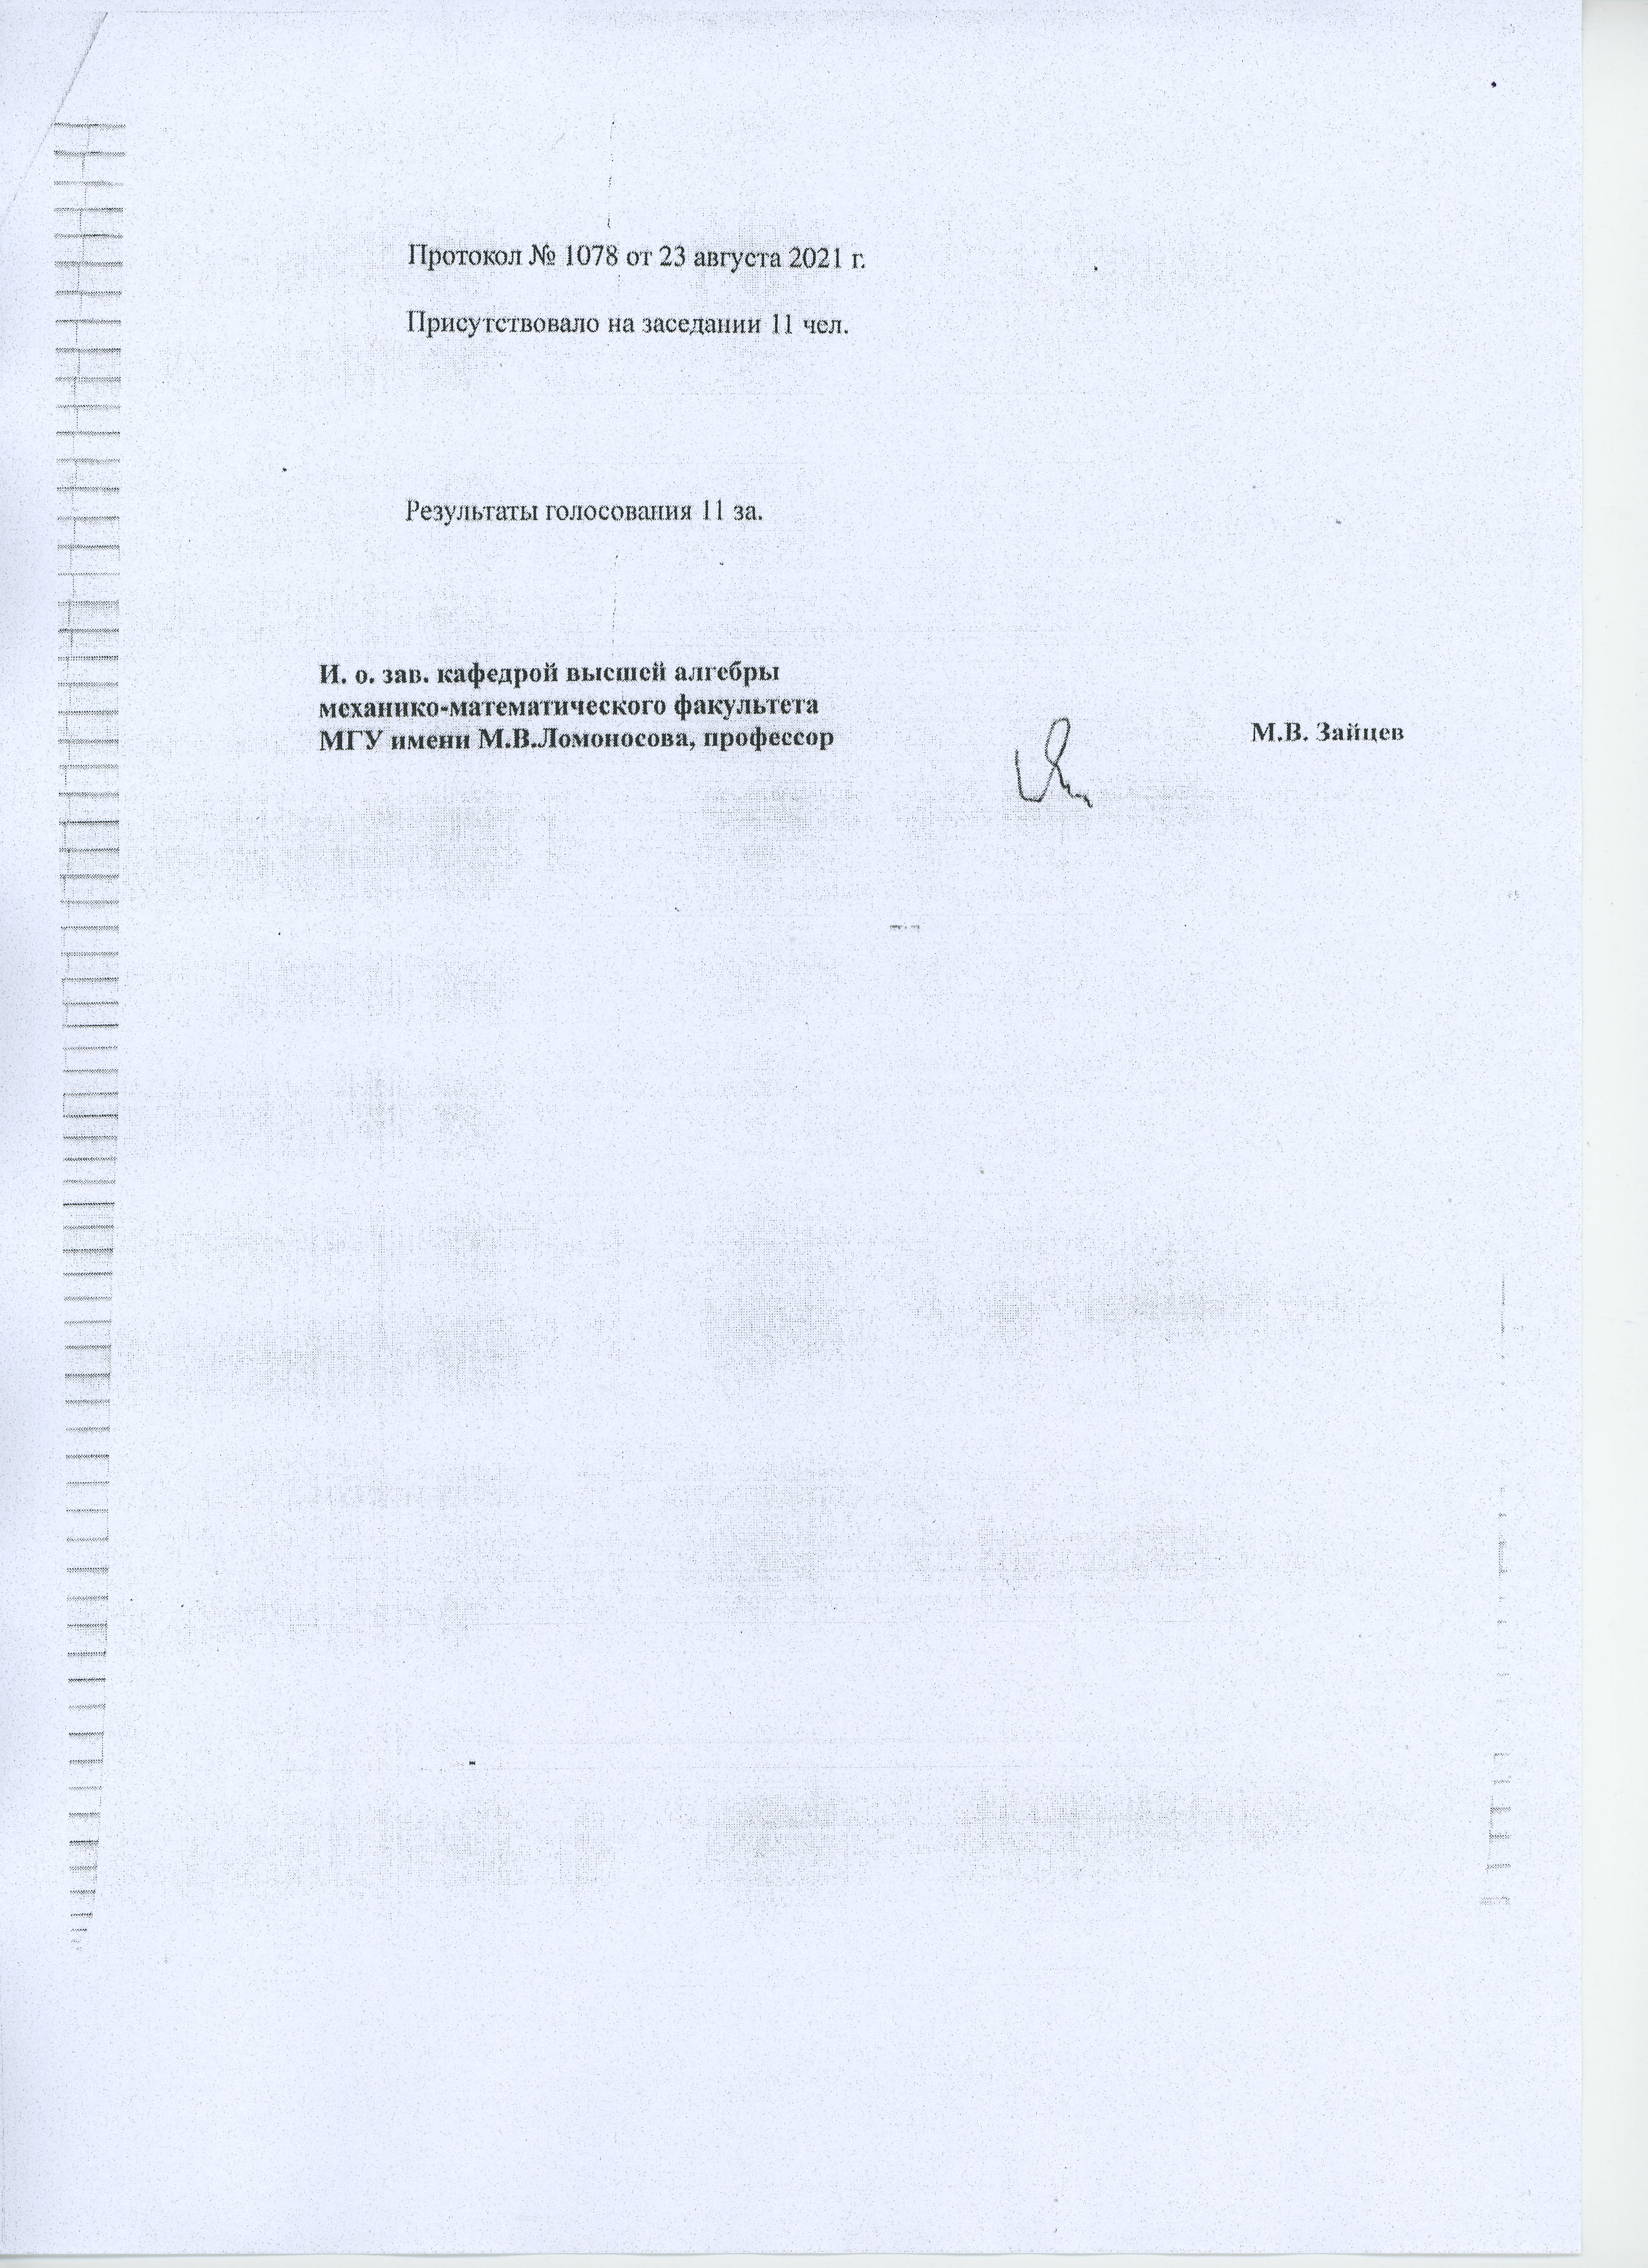
\includegraphics[width=0.75\linewidth]{kaf3}
\end{frame}

\begin{frame} % публикации на одной странице
% \begin{frame}[t,allowframebreaks] % публикации на нескольких страницах
    \frametitle{Основные публикации}
    \nocite{intsys20}%
    \nocite{pdm20}%
    \nocite{dm21}%
    \ifnumequal{\value{bibliosel}}{0}{
        \insertbiblioauthor
    }{
        \printbibliography%
    }
\end{frame}

\begin{frame}
    \frametitle{Участие в конференциях}
    \begin{itemize}
	\item \rom{26} Международная конференция студентов, аспирантов и молодых учёных <<Ломоносов>>, 2019 
	\item 10th Workshop on Current Trends in Cryptology (CTCrypt 2021).
    \end{itemize}
\end{frame}

\begin{frame}[plain, noframenumbering] % последний слайд без оформления
    \begin{center}
        \Huge
        Спасибо за внимание!
    \end{center}
\end{frame}
